%%% LaTeX Template: Two column article
%%%
%%% Source: http://www.howtotex.com/
%%% Feel free to distribute this template, but please keep to referal to http://www.howtotex.com/ here.
%%% Date: February 2011

%%% Preamble
\documentclass[	DIV=calc,%
							paper=a4,%
							fontsize=12pt,%
							onecolumn]{scrartcl}	 					% KOMA-article class

\usepackage{lipsum}													% Package to create dummy text
\usepackage[brazil]{babel}										% English language/hyphenation
\usepackage[protrusion=true,expansion=true]{microtype}				% Better typography
\usepackage{amsmath,amsfonts,amsthm}					% Math packages
\usepackage[pdftex]{graphicx}									% Enable pdflatex
\usepackage[svgnames]{xcolor}									% Enabling colors by their 'svgnames'
\usepackage[hang, small,labelfont=bf,up,textfont=it,up]{caption}	% Custom captions under/above floats
\usepackage{epstopdf}												% Converts .eps to .pdf
\usepackage{subfig}													% Subfigures
\usepackage{booktabs}												% Nicer tables
\usepackage{fix-cm}													% Custom fontsizes
\usepackage[utf8]{inputenc}
\usepackage[top=2.5cm, bottom=2.5cm, left=2.5cm, right=2.5cm]{geometry}
\usepackage[ddmmyyyy]{datetime}
\addto\captionsenglish{%
	\renewcommand\tablename{Tabela}
	\renewcommand\figurename{Figura}
} 
 

 
%%% Custom sectioning (sectsty package)
\usepackage{sectsty}													% Custom sectioning (see below)
\allsectionsfont{%															% Change font of al section commands
	\usefont{OT1}{phv}{b}{n}%										% bch-b-n: CharterBT-Bold font
	}

\sectionfont{%																% Change font of \section command
	\usefont{OT1}{phv}{b}{n}%										% bch-b-n: CharterBT-Bold font
	}



%%% Headers and footers
\usepackage{fancyhdr}												% Needed to define custom headers/footers
	\pagestyle{fancy}														% Enabling the custom headers/footers
\usepackage{lastpage}	

% Header (empty)
\lhead{}
\chead{}
\rhead{}
% Footer (you may change this to your own needs)

%% ====================================
%% ====================================
%% mude o rodape  do projeto
%% ====================================
%% ====================================

\lfoot{\footnotesize \texttt{Cabeamento estruturado} \textbullet ~Modelo de projeto}


\cfoot{}
\rfoot{\footnotesize página \thepage\ de \pageref{LastPage}}	% "Page 1 of 2"
\renewcommand{\headrulewidth}{0.0pt}
\renewcommand{\footrulewidth}{0.4pt}



%%% Creating an initial of the very first character of the content
\usepackage{lettrine}
\newcommand{\initial}[1]{%
     \lettrine[lines=3,lhang=0.3,nindent=0em]{
     				\color{DarkGoldenrod}
     				{\textsf{#1}}}{}}



%%% Title, author and date metadata
\usepackage{titling}															% For custom titles

\newcommand{\HorRule}{\color{DarkGoldenrod}%			% Creating a horizontal rule
									  	\rule{\linewidth}{1pt}%
										}

\pretitle{\vspace{-30pt} \begin{flushleft} \HorRule 
				\fontsize{50}{50} \usefont{OT1}{phv}{b}{n} \color{DarkRed} \selectfont 
				}

%% ====================================
%% ====================================
%% mude o titulo  do projeto
%% ====================================
%% ====================================

\title{Cabeamento Estruturado para Moura Contabilidade e Assessoria Ltda }					% Title of your article goes here

%% ====================================



\posttitle{\par\end{flushleft}\vskip 0.5em}

\preauthor{\begin{flushleft}
					\large \lineskip 0.5em \usefont{OT1}{phv}{b}{sl} \color{DarkRed}}
\author{Alysson Cristiano Estevam de Moura }  	% Author name goes here


\postauthor{\footnotesize \usefont{OT1}{phv}{m}{sl} \color{Black} 
					\\Universidade Tecnológica Federal do Paraná - Câmpus Cornélio Procópio 								% Institution of author
					\par\end{flushleft}\HorRule}

\date{}																				% No date




%%% Begin document
\begin{document}
\maketitle
\thispagestyle{fancy} 	
\thispagestyle{empty}		% Enabling the custom headers/footers for the first page 
% The first character should be within \initial{}




%% ====================================
%% ====================================
%% mude o resumo  do projeto
%% ====================================
%% ====================================

\initial{E}\textbf{ste documento consiste na elaboração de um projeto de cabeamento estruturado para a empresa Moura Contabilidade e Assessoria Ltda. O projeto apresenta a planta física, planta cabeada, topologia, memorial descritivo dos equipamentos passivos da rede, levantamento de quantidade/custo, Plano de Certificação e orçamento e o escopo do projeto.}


%% ====================================
\begin{figure}
	\centering
	\includegraphics{utfpr}
\end{figure}

\vspace{2cm}
\centerline{\textit{\textbf{\today}}}

\clearpage
    \renewcommand*\listfigurename{Lista de figuras}
\listoffigures

\renewcommand*\listtablename{Lista de tabelas}
\listoftables




\clearpage
\renewcommand{\contentsname}{Sumário}
\tableofcontents
\clearpage

%% ====================================
%% ====================================
%% Inicio do texto
%% ====================================
%% ====================================
\section{Introdução}

A empresa Moura Contabilidade e Assessoria Ltda atua na consultoria, gestão contábil e gestão tributária. Ela participa de todos os passos da administração de uma empresa, desde sua constituição até seu encerramento. Solucionam diversos problemas que surgem na rotina contábil empresarial. Também atuam na emissão de relatórios com o objetivo de auxiliar as empresas na tomada de decisões mais assertivas. Além disso, auxiliam com suporte para gestão tributária de forma a adequar a empresa as normas contábeis e legislação vigente.

A empresa possui o corpo funcional de: 2 Diretores, 4 Recepcionistas, 1 Assistente Administrativo, 2 Analistas de Sistemas, 4 Administradores e 10 Contadores.

Por se tratar de uma empresa nova, a instalação do cabeamento estruturado de redes será implantada de forma inicial após a criação do projeto.

\subsection{Benefícios}
Os principais benefícios que serão obtidos com o cabeamento estruturado serão:
\begin{itemize}
\item Fornecimento de serviços básicos de rede de computadores para a empresa
\item Aumento e melhoria de segurança da informação
\item Compartilhamento seguro de arquivos entre os computadores da rede
\item Sistema de backup e redundância com possibilidade de Disaster Recovery
\item Controle de acesso
\item Internet de alta velocidade compartilhada entre os computadores da rede
\item Melhoria do desempenho da rede
\item Maior facilidade de identificação de erros na rede e com isso manutenção mais rápida
\item Facilidade de gerenciamento do ambiente de TI da empresa
\end{itemize}
	
\subsection{Organizações Envolvidas}
Tabela com a relação das organizações envolvidas:

\begin{table}[]
	\begin{tabular}{|l|l|}
		\hline
		\multicolumn{1}{|c|}{\textbf{Profissional/Empresa}} & \multicolumn{1}{c|}{\textbf{Serviço}}                         \\ \hline
		Provedor de Internet 1                              & Serviço de acesso à Internet                                  \\ \hline
		Provedor de Internet 2                              & Serviço de acesso à Internet para redundância                 \\ \hline
		Engenheiro Eletricista                              & Instalações elétricas demandadas                              \\ \hline
		Analista de Compras                                 & Orçamentos e compras de equipamentos                          \\ \hline
		Projetista de Rede                                  & Projeto da rede física e lógica                               \\ \hline
		Instalador da Rede                                  & Profissional ou equipe para instalar a rede física            \\ \hline
		Telecom Local                                       & Instala/remaneja os troncos telefônicos                       \\ \hline
		Empresa de Telefonia                                & Profissional ou equipe para instalar PABX e cabos telefônicos \\ \hline
		ANATEL                                              & Órgão de fiscalização de Telecomunicação                      \\ \hline
	\end{tabular}
\end{table}


\section{Requisitos}

Nesta seção serão apresentados os principais requisitos do projeto de cabeamento estruturado da rede:	

\begin{itemize}				
\item A rede deverá permitir acessos simultâneos a Internet, para isso contará com largura de banda suficientemente alta para ser compartilhada por vários PCs
\item A rede deverá permitir o compartilhamento de arquivos na rede, para isso utilizará de um servidor de arquivos com alta capacidade de armazenamento 
\item A rede deverá permitir o compartilhamento de impressoras, para isso deverão ser configurados pontos de rede para o compartilhamento de impressoras.		
\item A rede deverá bloquear o acesso a sites com conteúdos indesejáveis, para isso possuirá um servidor proxy para filtrar conteúdos indesejáveis de forma a atender a política da empresa.
\item A rede deverá ter garantia de funcionamento e confiabilidade do acesso a Internet, para isso possuirá link redundante de Internet, tanto no meio físico quanto na operadora, de forma a garantir a disponibilidade.
\item A rede possuirá servidores de backup com os softwares necessários para Disaster Recover, com isso será garantida a cópia de segurança dos dados e com possibilidade de rápida recuperação.
\item A rede deverá garantir a segurança das informações utilizando um firewall contra intrusos, para isso utilizará o mesmo servidor proxy para acesso a internet.
\end{itemize}

\section{Usuários e Aplicativos}
Nesta seção serão descritos os profissionais que trabalham na empresa e que farão uso do cabeamento estruturado. Com isso será apresentado o tipo de usuário e os aplicativos que ele mais utiliza. 

\subsection{Usuários}

A tabela \ref{tab:usuarios} mostra os Usuários com os aplicativos mais utilizados.

\begin{table}[t]
	\begin{tabular}{|p{5cm}|p{11cm}|}
		\hline
		\multicolumn{1}{|c|}{\textbf{Usuário}} & \multicolumn{1}{c|}{\textbf{Aplicativos mais utilizados}}                                                                           \\ \hline
		Diretor 1 a 2 & Windows 10, Microsoft Office Professional 2016, Microsoft Outlook e Mozilla Firefox 
		\\ \hline
		Recepcionista 1 a 4 & Windows 10, Microsoft Office Professional 2016 e Microsoft Outlook                                                               \\ \hline
		Assistente Administrativo & Windows 10, Microsoft Office Professional 2016, Microsoft Outlook e Mozilla Firefox 
		\\ \hline
		Analista de Sistemas 1 & Windows Server 2016, SQL Server 2017, Microsoft System Center Configuration Manager, Cisco IOS, Mozilla Firefox e Microsoft Outlook 
		\\ \hline
		Analista de Sistemas 2 & Windows 10, Microsoft Office Professional 2016, Mozilla Firefox, Microsoft Outlook, softwares de desenvolvimento                    
		\\ \hline
		Administrador 1 a 4 & Windows 10, Microsoft Office Professional 2016, Microsoft Outlook, Microsoft Teams e Mozilla Firefox 
		\\ \hline
		Contadores 1 a 10 & Windows 10, Microsoft Office Professional 2016, Mozilla Firefox e programas fiscais 
		\\ \hline
	\end{tabular}
	\caption{Tabela Usuários}
	\label{tab:usuarios}
\end{table}

O Diretor é responsável por planejar, organizar e controlar as atividades da empresa, além de traçar estratégias e métodos de trabalho com o objetivo de desenvolve-lá. É auxiliado pelos Administradores na tomada de decisões. 

Os Administradores são responsáveis por organizar, planejar e orientar o uso dos recursos financeiros, físicos, tecnológicos e humanos da empresa, buscando soluções para todo tipo de problema administrativo. Eles se relacionam com todas as áreas dentro de uma empresa e auxiliam o Diretor nas tomadas de decisões.

O Assistente Administrativo é responsável por ajudar os diretores com tarefas rotineiras de cunho administrativo.
Os Recepcionistas são responsáveis pelo atendimento telefônico, recepção de clientes, anotação de recados, envio e controle de correspondências, etc.

O Analista de Sistemas 1 é responsável pelo gerenciamento de redes, segurança dos sistemas, gerenciamento de servidores, e qualquer outra atividade relacionada ao suporte de Tecnologia da Informação.

O Analista de Sistemas 2 é responsável pelo desenvolvimento de softwares necessários para a empresa, bem como a página Web da empresa.

Os Contadores atuam no atendimento aos clientes para fins de suporte contábil, econômico e financeiro. São responsáveis por registrar, organizar, demonstrar, analisar e acompanhar as modificações do patrimônio em virtude da atividade econômica ou social que a empresa exerce no contexto econômico.

\subsection{Aplicativos}

A tabela \ref{tab:aplicativos} apresenta os aplicativos mais utilizados e seu nível crítico de uso:

\begin{table}[]
	\begin{tabular}{|p{6cm}|p{10cm}|}
		\hline
		\multicolumn{1}{|c|}{\textbf{Aplicativo}} & \multicolumn{1}{c|}{\textbf{Uso}}                                           \\ \hline
		Microsoft Windows 10                      & Sistema operacional utilizado nas estações de trabalho                      \\ \hline
		Microsoft Office Professional 2016        & Suíte de aplicativos para criação de textos, planilhas, apresentações, etc  \\ \hline
		Microsoft Outlook                         & Aplicativo para gerenciamento de emails                                     \\ \hline
		Mozilla Firefox 68.4.1                    & Navegador utilizado pelos funcionários da empresa                           \\ \hline
		Microsoft Windows Server 2016             & Sistema operacional utilizado no servidor da empresa                        \\ \hline
		Microsoft SQL Server 2017                 & Banco de dados utilizado no servidor da empresa                             \\ \hline
		System Center Configuration Manager       & Programa para gerenciamento distribuído de todos os computadores da empresa \\ \hline
		Cisco IOS                                 & Sistema operacional dos equipamentos de rede da empresa                     \\ \hline
		Programas fiscais                         & Programas de uso contábil                                                   \\ \hline
		Softwares de desenvolvimento              & IDEs de desenvolvimento, compiladores, ferramentas gráficas, etc            \\ \hline
	\end{tabular}
	\caption{Tabela Aplicativos}
	\label{tab:aplicativos}
\end{table}

A empresa conta com dois servidores, um principal e um secundário. O servidor principal será utilizado no controle de usuário, armazenamento de arquivos, compartilhamento de sistemas, backup, replicação e outros serviços necessário para o funcionamento da empresa. Todo o armazenamento do servidor principal será migrado de forma redundante para o servidor secundário. Assim, caso ocorra algum problema com o servidor principal, não haverá perdas para a empresa.


\section{Estrutura predial existente}

Trata-se de uma estrutura predial nova onde será implantado o cabeamento estruturado horizontal. De um modo geral, cada área respeitará a Norma possuindo no mínimo 2 tomadas de telecomunicações, para um máximo de 10m2. Também manterá a distância mínima de 30cm entre tomadas de superfície e piso. Os cabos possuirão a distância máxima de 5m entre a tomada e o equipamento. A planta baixa (figura \ref{planta2d}) se encontra em anexo no fim do projeto. 


\section{Planta Lógica - Elementos estruturados}

\subsection{Planta cabeada}

O cabeamento utiliza cabos UTP Categoria 6 para conexão dos equipamentos, LAN Gigabit, equipamentos de alta confiabilidade e protocolo TCP/IP. O acesso à rede externa é provido por duas operadoras de telefonia utilizando fibra ótica com o objetivo de garantir disponibilidade da rede. A instalação será feita pelas operadoras e a configuração/manutenção dos equipamentos terá SLA mínimo de duas horas, 24 X 7. O link possuirá largura de banda de 300Mbps com possibilidade de expansão se necessário. 

A rede possuirá 64 pontos de rede (PT000 até PT063), sendo distribuída da seguinte forma:

\begin{itemize}
\item Sala de Recepção: 10 pontos de rede
\item Escritório 1 a 10: 2 pontos de rede por escritório = 20 pontos
\item Direção Geral: 8 pontos de rede
\item Direção Administrativa 1 a 4: 4 pontos por direção administrativa = 16 pontos de rede
\item Sala de Reunião: 6 pontos de rede
\item Sala de TI: 4 pontos de rede
\end{itemize}

A planta baixa cabeada (figura \ref{planta2d_cabeada}) se encontra em anexo no fim do projeto. 

\subsection{Topologia}

Basicamente a rede possui um roteador que é o Gateway padrão para a conexão com a internet. A rede também possui dois Switches de 36 portas cada, onde o Switch 1 engloba os pontos de rede PT000 a PT031 e o Switch 2 engloba os pontos de rede PT032 a PT063. O roteador também é conectado aos Switches e aos Servidores 1 e 2. O Terminal serve para operar os servidores localmente. 

A figura \ref{topologia} mostra a topologia a ser implementada.

\begin{figure}
	\centering
	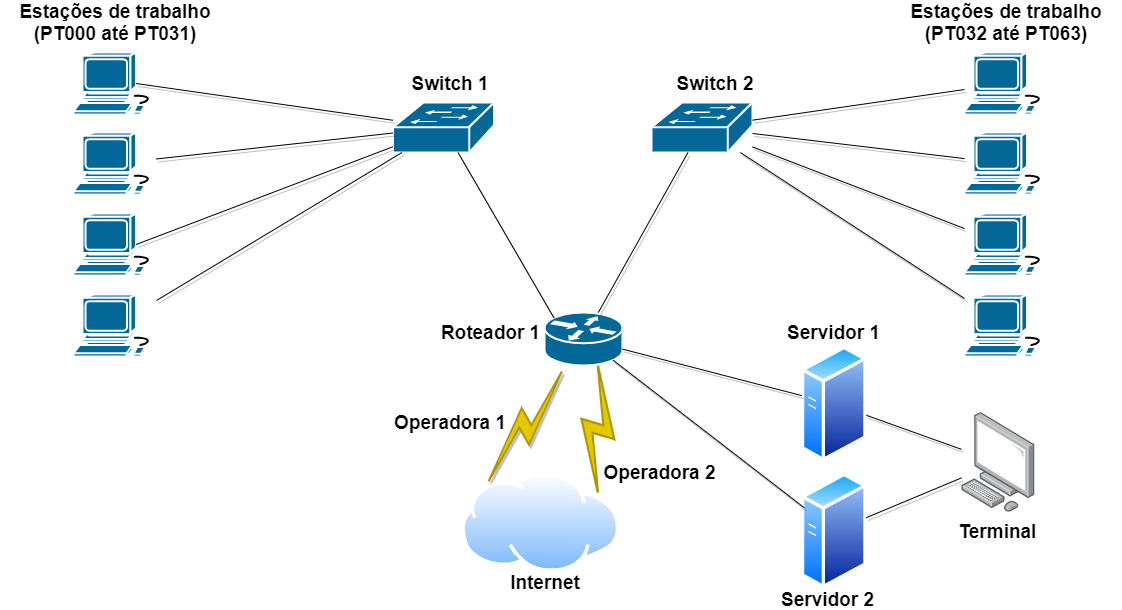
\includegraphics[width=\textwidth]{topologia}
	\caption{Diagrama do projeto lógico}
	\label{topologia}
\end{figure}


\subsection{Encaminhamento}

O encaminhamento utilizado será canaleta X2 Adesivada em todo o cabeamento estruturado.

\subsection{Memorial descritivo}

O cálculo da quantidade de cabos foi feito utilizando a seguinte fórmula empírica: 

\begin{equation}
Qc = \frac{(Ponto Mais Proximo + Ponto Mais Distante + 4*PeDireito)*QtdPontos*1,1}{2}
\end{equation}

\begin{equation}
Qc = \frac{(1 + 49 + 4*3)*64*1,1}{2} = 2182,4 m
\end{equation}

A tabela \ref{tab:passivos} apresenta os componentes passivos do cabeamento.

\begin{table}[]
	\begin{tabular}{|l|l|l|}
		\hline
		\multicolumn{1}{|c|}{\textbf{Equipamento Passivo}} & \multicolumn{1}{c|}{\textbf{Fabricante}} & \multicolumn{1}{c|}{\textbf{Quantidade}} \\ \hline
		Rack 44 U Fechado                                  & Furukawa                                 & 1                                        \\ \hline
		Patch Panel 36 Portas CAT 6                        & Furukawa                                 & 2                                        \\ \hline
		Cabo UTP CAT 6 - 305 m                             & Furukawa                                 & 7                                        \\ \hline
		Cabo UTP CAT 6 - 100 m                             & Furukawa                                 & 1                                        \\ \hline
		Patch Cords CAT 6 - 2 m                            & Furukawa                                 & 36                                       \\ \hline
		Patch Cords CAT 6 - 1,5m                              & Furukawa                                 & 36                                       \\ \hline
		Tomadas (outlet) CAT6 c/ 1 ponto RJ45              & WEG                                      & 36                                       \\ \hline
	\end{tabular}
\caption{Tabela Componentes Passivos}
\label{tab:passivos}
\end{table}

\subsection{Identificação dos cabos}
Explique como os cabos serão identificados em seu projeto. Coloque uma relação dos cabos instalados e identificados.

\section{Implantação}
Estabeleça um cronograma de implantação:
Remoção de equipamentos existentes (destino para descarte), instalação dos condutores, instalação dos cabos, 
identificação dos cabos, montagem dos racks, certificação, etc... Crie atividades e estabeleça o tempo de execução. Se for um projeto real, indique também quais os responsáveis pela execução do projeto e de cada uma das etapas.

Defina marcas (e padrões) e fornecedores se for o caso. Atenção a contratados e subcontratados para a realização das atividades. Estabeleça a responsabilidade de execução da atividade e também da validação dela.

Utilize algum software para gerear o cronograma. Excel,etc. O fundamental é dividir em etapas, descrever e estimar o tempo de cada uma delas.

Segue uma relação de ferramentas:
http://asana.com/, 
https://trello.com/, 
http://www.ganttproject.biz/, 
http://www.orangescrum.org/. 

\section{Plano de certificação}
Quais seriam as etapas para a certificação? 
Quais os locais e horários para execução da certificação na rede? Toda rede será certificada?
Como os testes seriam executados?
Quais relatórios de certificação serão (ou deveriam ser) entregues? 

\section{Plano de manutenção}

Revisões periódicas na rede, emissão de certificados para novos pontos.

\subsection{Plano de expansão}
Existe um plano de expansão? Quantos novos pontos poderão ser acrecidos na rede, antes de migração de equipamentos na camada 2? Se houver expansão, quais equipamentos deverão ser direcionados para as estremidades da rede? 

\section{Risco}
Enumerar e explicar os riscos do projeto.

\section{Orçamento}

A tabela \ref{tab:orcPassivos} apresenta o orçamento dos equipamentos passivos.

\begin{table}[]
	\begin{tabular}{|l|l|l|l|l|}
		\hline
		\multicolumn{1}{|c|}{\textbf{Equipamento Passivo}} & \multicolumn{1}{c|}{\textbf{Fabricante}} & \multicolumn{1}{c|}{\textbf{Qt}} & \textbf{Preço} & \textbf{Total (R\$)} \\ \hline
		Rack 44 U Fechado                                  & Furukawa                                 & 1                                & 3495,00        & 3495,00              \\ \hline
		Patch Panel 36 Portas CAT 6                        & Furukawa                                 & 2                                & 255,00         & 510,00               \\ \hline
		Cabo UTP CAT 6 - 305 m                             & Furukawa                                 & 7                                & 670,00         & 4690,00              \\ \hline
		Cabo UTP CAT 6 - 100 m                             & Furukawa                                 & 1                                & 350,00         & 350,00               \\ \hline
		Patch Cords CAT 6 - 2 m                            & Furukawa                                 & 36                               & 28,00          & 1008,00              \\ \hline
		Patch Cords CAT 6 - 1,5m                           & Furukawa                                 & 36                               & 31,00          & 1116,00              \\ \hline
		Tomadas (outlet) CAT6 c/ 1 ponto RJ45              & WEG                                      & 36                               & 77,00          & 2772,00              \\ \hline
	\end{tabular}
\caption{Tabela de Orçamento dos Equipamentos Passivos}
\label{tab:orcPassivos}
\end{table}

A tabela \ref{tab:orcEncaminhamentos} apresenta o orçamento dos equipamentos passivos.

\begin{table}[]
	\begin{tabular}{|l|l|l|l|l|}
		\hline
		\multicolumn{1}{|c|}{\textbf{Encaminhamento}} & \multicolumn{1}{c|}{\textbf{Fabricante}} & \multicolumn{1}{c|}{\textbf{Qt}} & \textbf{Preço} & \textbf{Total (R\$)} \\ \hline
		Canaleta X2 Adesivada                         & Dutoplast                                & 36                               & 31,00          & 1116,00              \\ \hline
		Acabamento X2                                 & Dutoplast                                & 36                               & 5,00           & 180,00               \\ \hline
	\end{tabular}
	\caption{Tabela de Orçamento dos Encaminhamentos}
	\label{tab:orcEncaminhamentos}
\end{table}

A tabela \ref{tab:orcAtivos} apresenta os equipamentos ativos do cabeamento estruturado.

\begin{table}[]
	\begin{tabular}{|l|l|l|l|l|}
		\hline
		\multicolumn{1}{|c|}{\textbf{Equipamento Ativo}} & \multicolumn{1}{c|}{\textbf{Fabricante}} & \multicolumn{1}{c|}{\textbf{Qt}} & \textbf{Preço} & \textbf{Total (R\$)} \\ \hline
		Switch 36 Portas                                 & Sun Oracle                               & 2                                & 1360,00        & 2720,00              \\ \hline
		Roteador RV340                                   & Cisco                                    & 1                                & 2242,00        & 2242,00              \\ \hline
		Servidor PowerEdge T140                          & Dell                                     & 2                                & 3600,00        & 7200,00              \\ \hline
	\end{tabular}
\caption{Tabela de Orçamento dos Equipamentos Ativos}
\label{tab:orcAtivos}
\end{table}

\section{Recomendações}
Observações e recomendações para o cliente.

\section{Referências bibliográficas}
Utilize o mendley, o jabref ou diretamente o bibtex para gerenciar suas referências biliográficas. As referências são criadas automaticamente de acordo com o uso no texto.

Exemplo: Redes de computadores, segundo \cite{t2013} é considerada..... Já \cite{kurose2010} apresenta uma versão...

Analisando os pressupostos de \cite{ref3} e \cite{ref4} concluimos que....


\renewcommand\refname{} %%Referências bibliográficas}  
\bibliographystyle{ieeetr}
\bibliography{referencias}  

%% ***********************************************************************
%% === remover daqui =====================================================
%% ***********************************************************************
=================================================
\section{Elementos textuais - Alguns exemplos}

Esta seção apresenta exemplos de elementos textuais. \textbf{Remova-a da versão final do texto}.


\subsection{Colocar elementos em itens}

Texto antes da lista

\begin{itemize}
	\item First item in a list 
	\item Second item in a list 
	\item Third item in a list
\end{itemize}

\subsubsection{Uma subseção de terceiro nivel}

Exemplo de uma subseção

\subsection{Tabelas}

Utilize o site http://www.tablesgenerator.com/ para elaborar as tabelas de seu trabalho.
Para adicionar uma tabela utilize: a tag input, passando o arquivo da tabela como parametro

\input{tab2}

Dentro do arquivo você deve definir o label e pode utilizá-lo para referenciar. Exemplo:
Na tab \ref{tab2} temos a relação de ....


Você também pode modificar a tabela manualmente, incluindo, por exemplo h! dentro de sua definição. Veja no exemplo tab2.tex

\subsection{Figuras}

As figuras podem ser no formato PDF, JPG, PNG. Você pode referenciá-las da mesma maneira que tabelas. Exemplo: A figura \ref{fig1} apresenta.....

Não se preocupe o local em que a figura será renderizada em seu texto. Preocupe-se em criar referência para ela, ou seja, toda figura e tabela deve conter pelo menos uma referência no texto.

\begin{figure}
\centering
\includegraphics[width=\textwidth]{fig1}
\caption{Exemplo de figura com escala horizontal}
\label{fig1}
\end{figure}


\begin{figure}
	\centering
	\includegraphics[]{fig2}
	\caption{Exemplo de figura sem escala}
	\label{fig2}
\end{figure}

Você pode rotacionar figuras também. Para isso utilize o parâmetro angle=-90. Repare que a escala da figura foi modificada pelo parametro height. Você também pode utilizar scale

\begin{figure}
	\centering
	\includegraphics[height=\textwidth,angle=-90]{fig3}
	\caption{Exemplo de figura rotacionada}
	\label{fig3}
\end{figure}

\begin{figure}
	%	\centering
	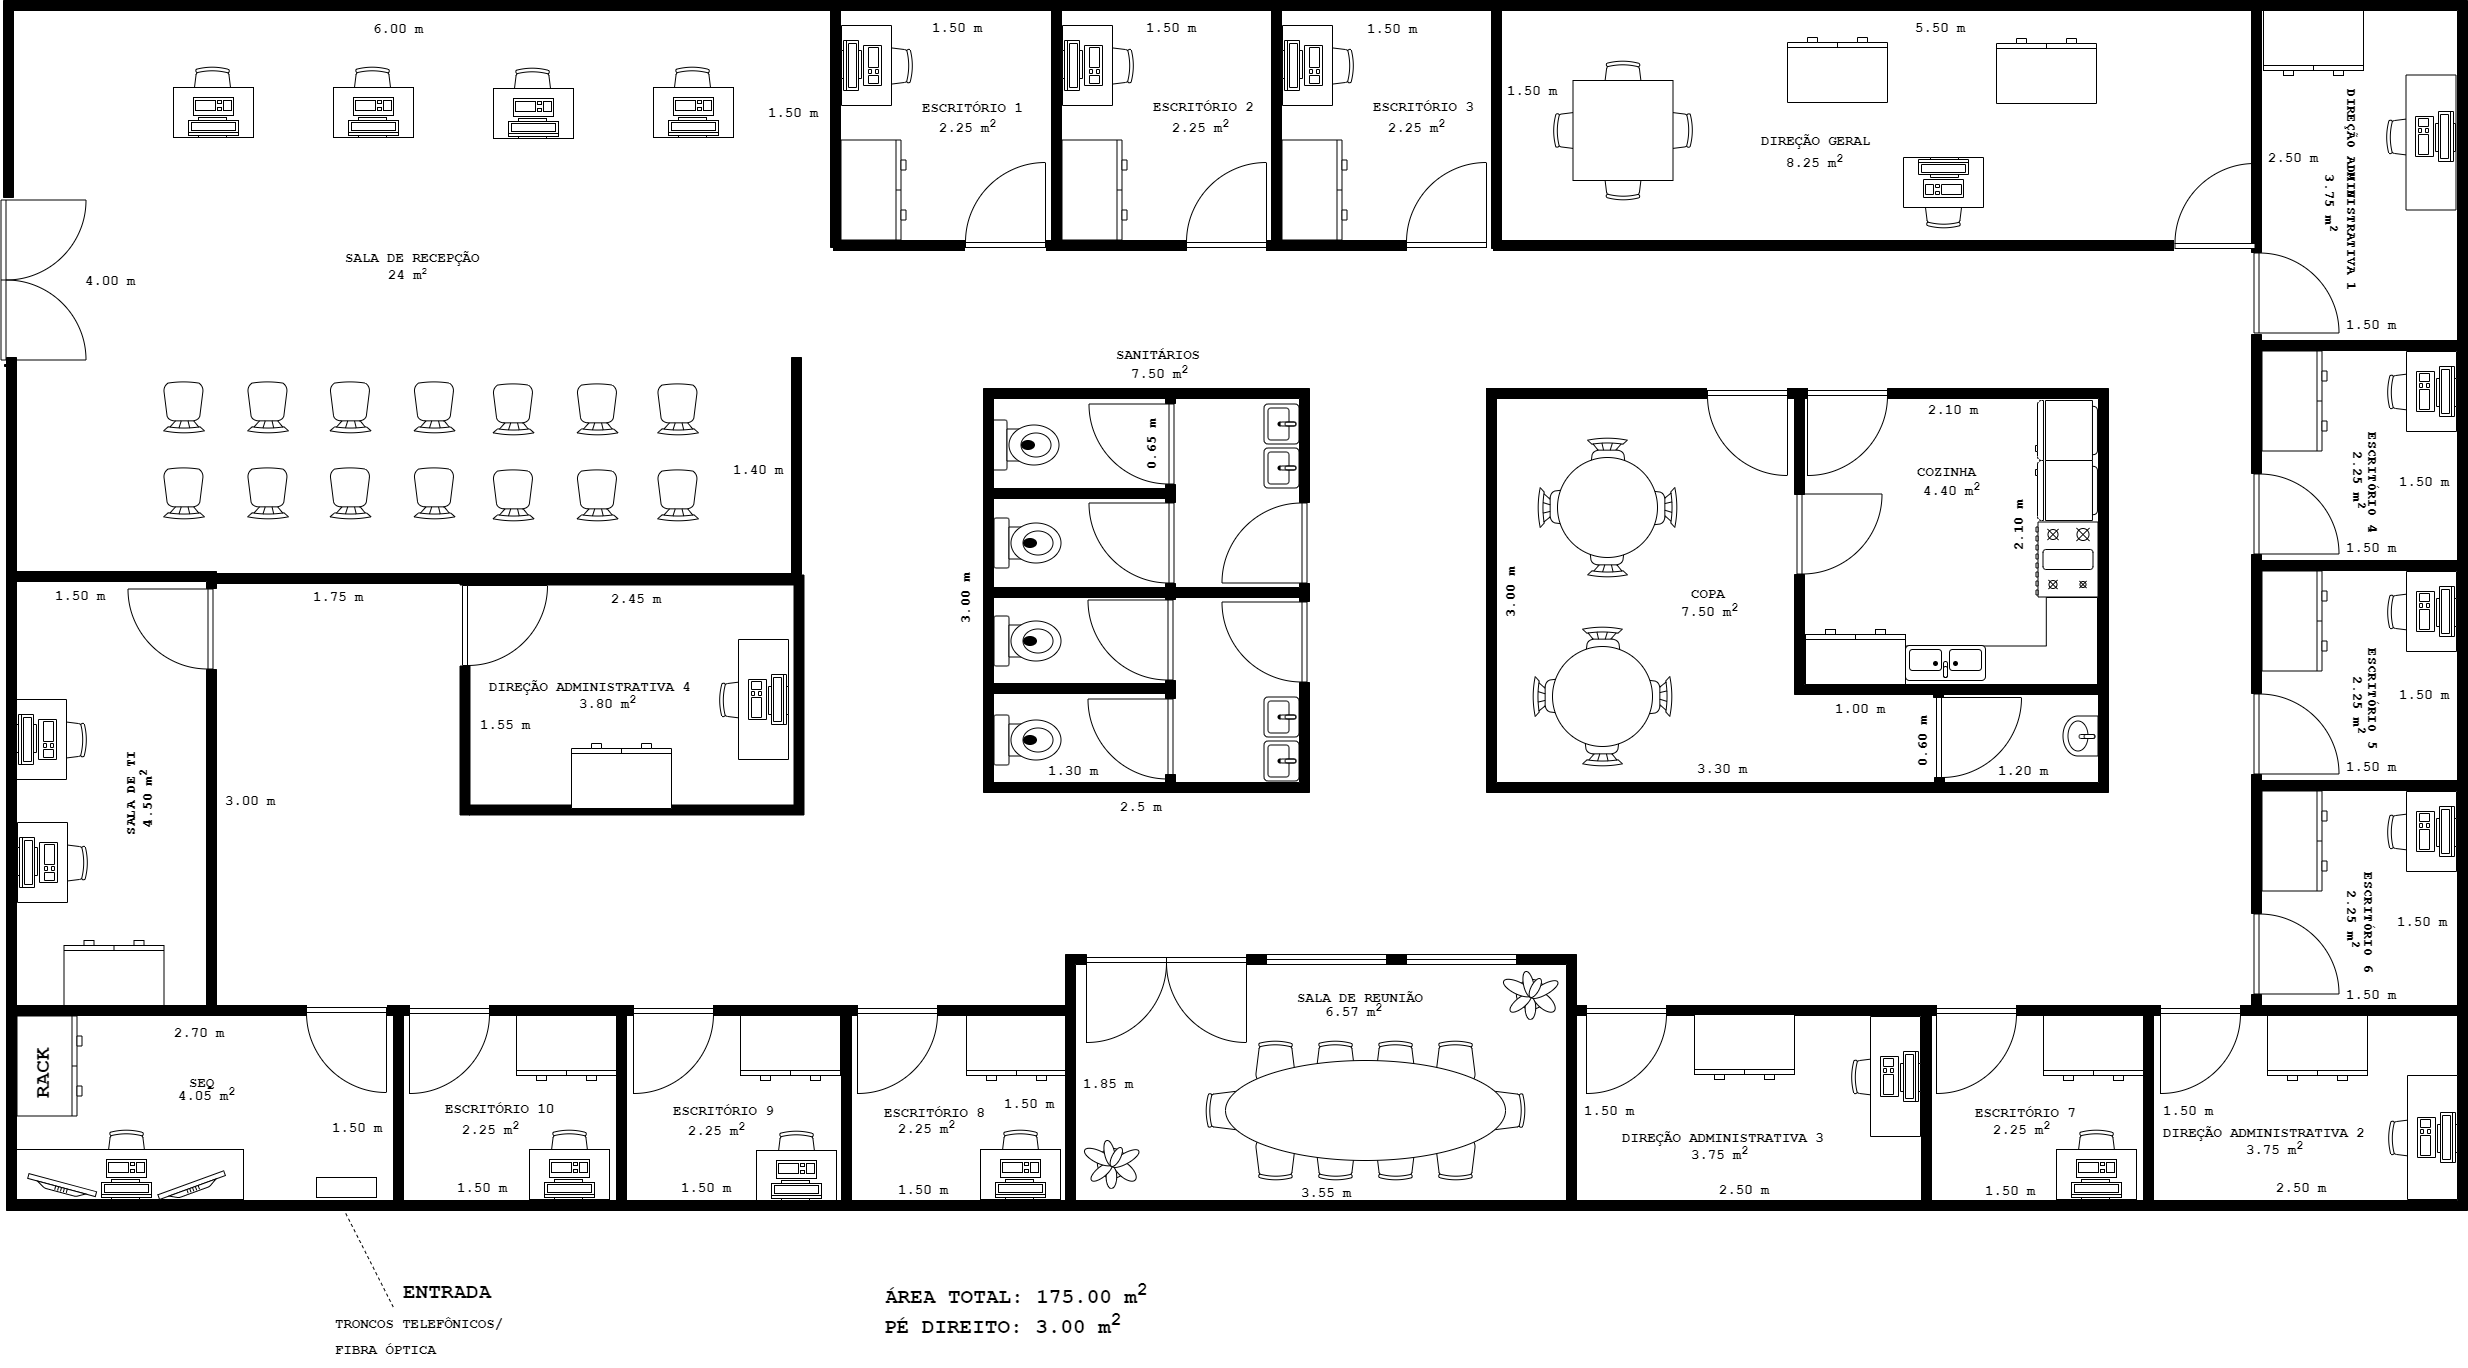
\includegraphics[height=\textwidth,angle=-90,scale=0.8]{planta2d}
	\caption{Planta baixa da estrutura predial}
	\label{planta2d}
\end{figure}

\begin{figure}
	%	\centering
	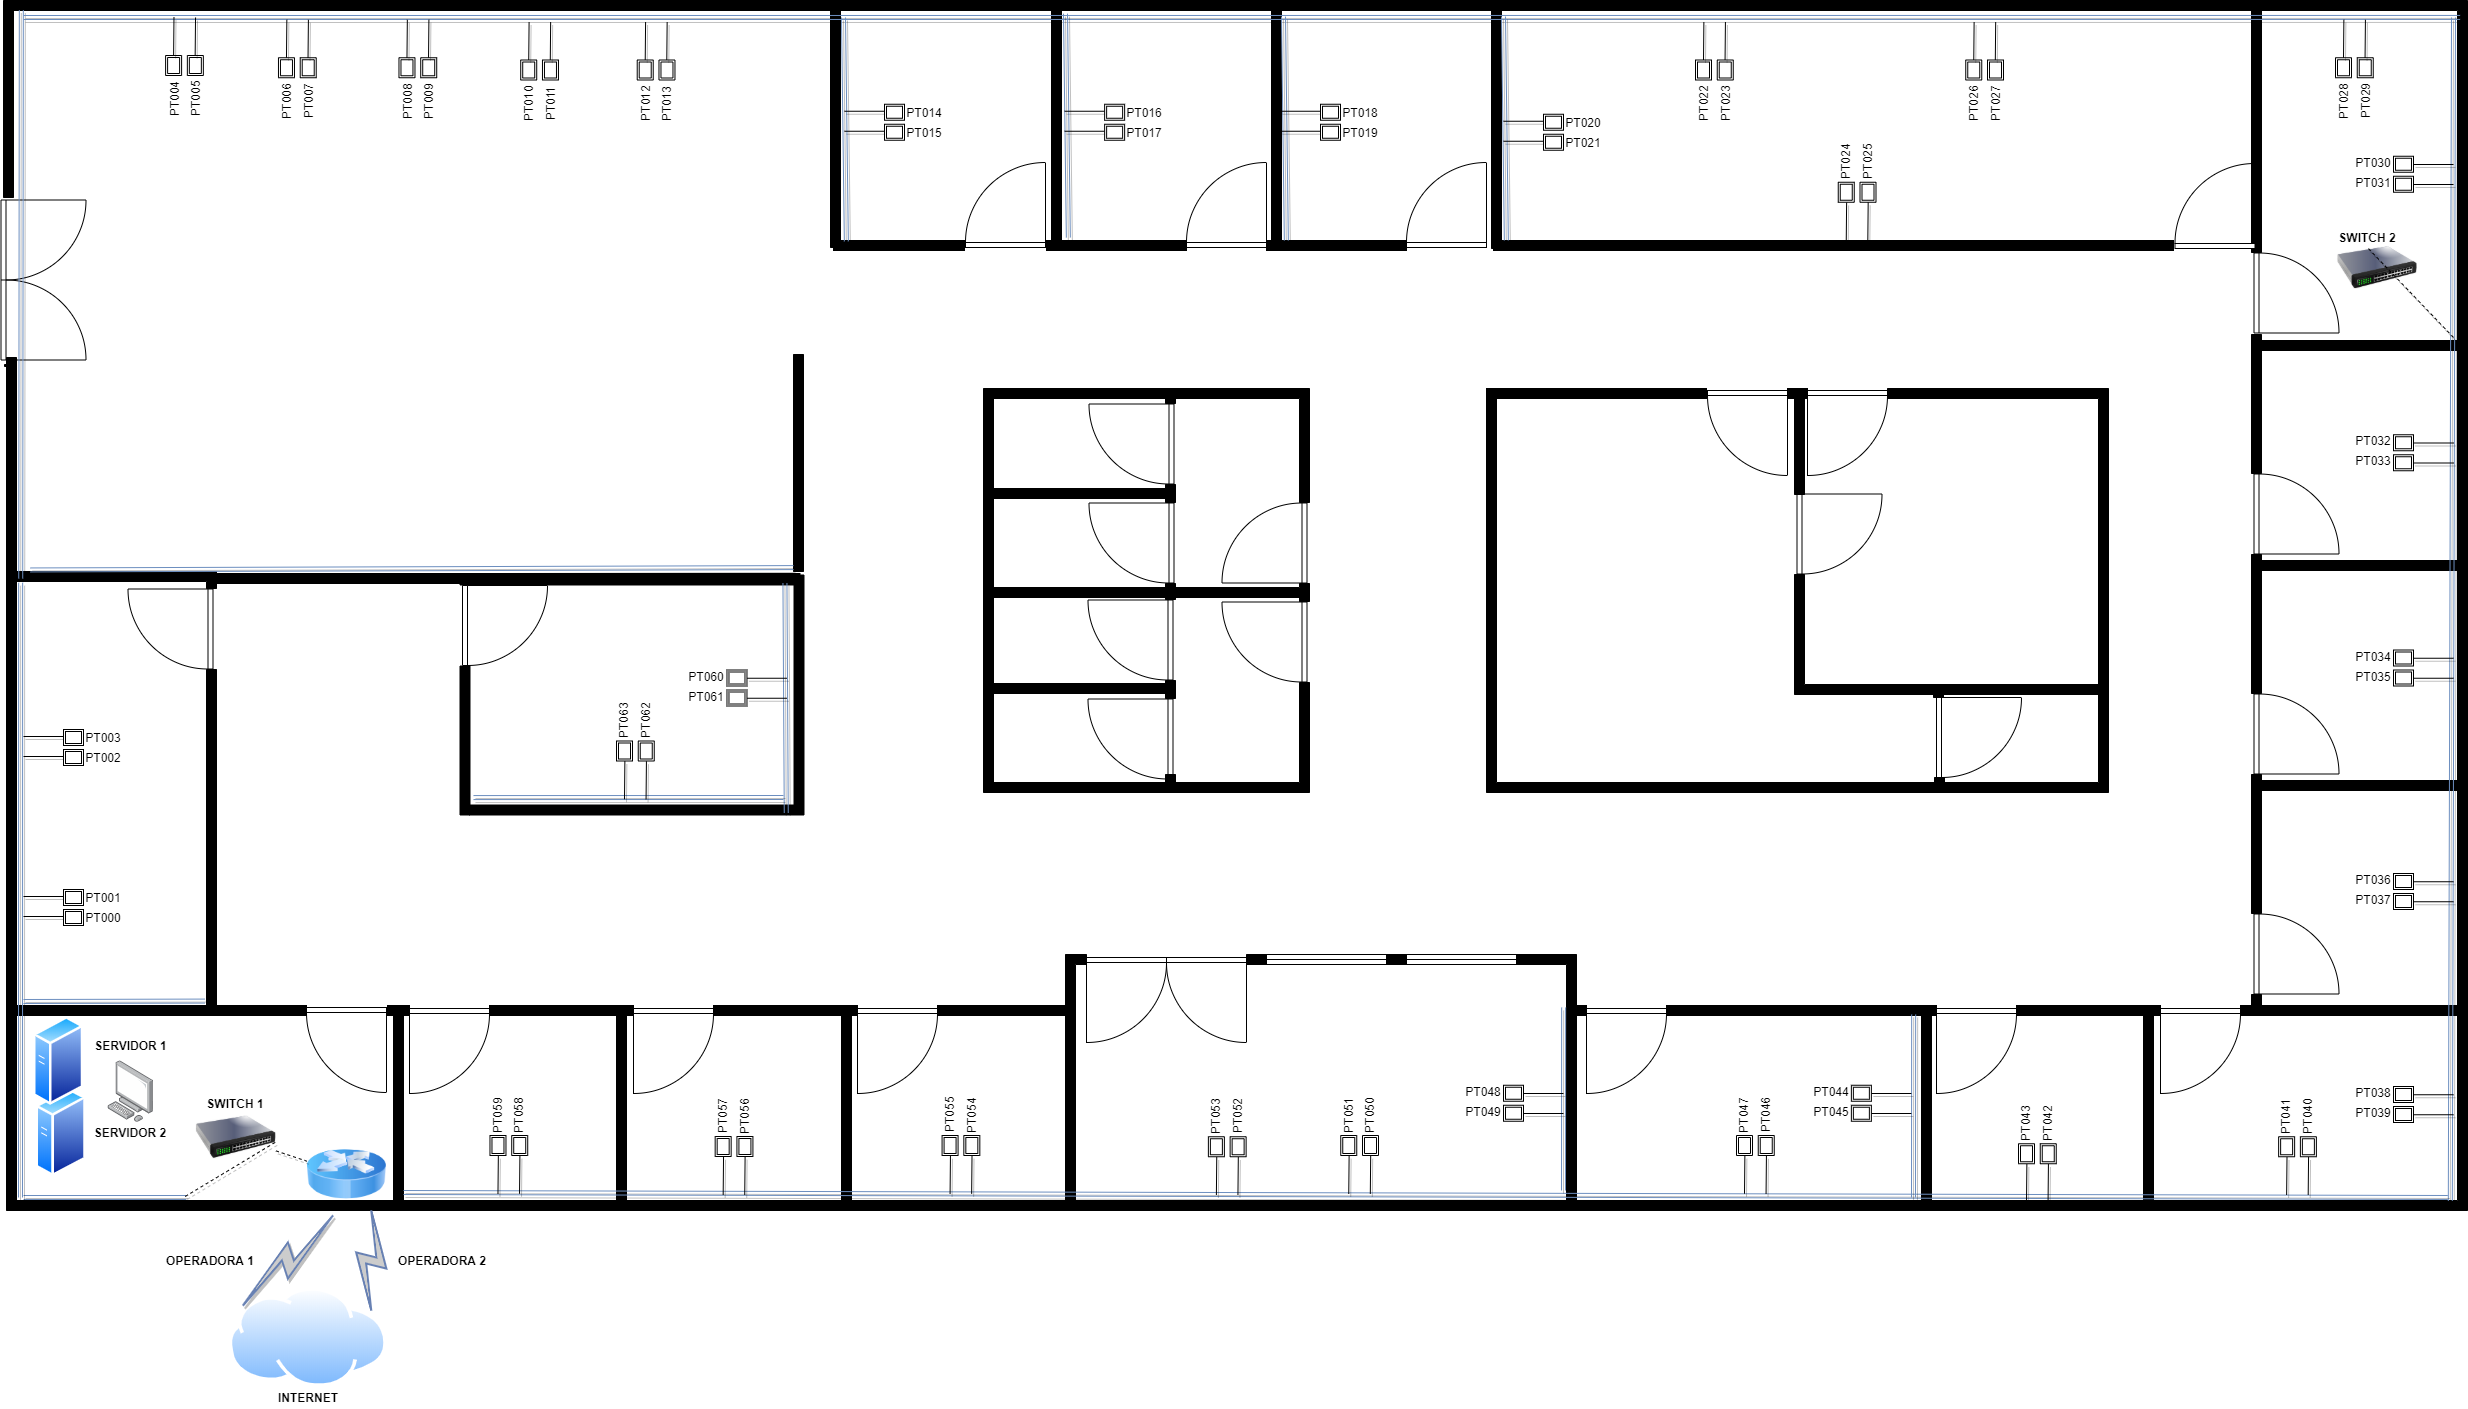
\includegraphics[height=\textwidth,angle=-90,scale=0.8]{planta2d_cabeada}
	\caption{Planta baixa cabeada}
	\label{planta2d_cabeada}
\end{figure}

Você também pode inserir páginas de outro tamanho em seu texto. Isto irá ajudar a inserir imagens maiores, como as desenvolvidas em CAD. Segue um exemplo na figura \ref{fig4} e figura \ref{fig5}.


%inicio dos comandos para criar uma nova pagina A3
\clearpage
\KOMAoptions{paper=a3, pagesize}
\recalctypearea

\begin{figure}
	\centering
	\makebox[\textwidth][c]{
		\includegraphics[height=\textheight]{fig3}}
	\caption{Exemplo de figura inserida em uma página A3}
	\label{fig4}
\end{figure}

%Retornar ao formato A4
\clearpage
\KOMAoptions{paper=a4, pagesize}
\recalctypearea
%-- reinicio em A4 


%inicio dos comandos para criar uma nova pagina A3 horizontal
\clearpage
\KOMAoptions{paper=a3, paper=landscape, DIV=20}
\recalctypearea

	
\begin{figure}
%	\centering
	\noindent\makebox[\textwidth][c]{
		\includegraphics[width=\textwidth]{fig3}
	}
	\caption{Exemplo de figura inserida em uma página A3 no formato horizontal}
	\label{fig5}
\end{figure}

%Retornar ao formato A4
\clearpage
\KOMAoptions{paper=a4, paper=portrait, DIV=15}
\recalctypearea
%-- reinicio em A4 


\subsubsection{Resumo gráfico}

Você pode optar por fazer um resumo no formato de mapa mental/conceitual. 
Aqui foi utilizado o site https://app.mindmup.com para gerar o mapa.

Para utilizar o resumo gráfico, remova o texto da seção resumo (linha 137) e inclua o código para inserir a figura, conforme figura \ref{fig6}

\begin{figure}[h]
	\centering
	\includegraphics[width=\textwidth,height=5cm,keepaspectratio]{fig4}
	\caption{Exemplo de resumo gráfico}
	\label{fig6}	
\end{figure}

%% ***********************************************************************
%% === ate aqui    =====  ================================================
%% ***********************************************************************

\end{document}